% =====================================================================
%  Manuscript for Biomedical Signal Processing and Control (Elsevier)
%  Official elsarticle class, preprint, 12pt, elsarticle-num.bst. Revision R2.
%  Every number traces to reports/ (see revision/response_bspc_r2.md).
% =====================================================================
\documentclass[preprint,12pt]{elsarticle}
\usepackage[T1]{fontenc}
\usepackage{lmodern}
\usepackage{amsmath,amssymb}
\usepackage{graphicx}
\usepackage{booktabs}
\usepackage{multirow}
\usepackage{textcomp}
\usepackage[hidelinks]{hyperref}
\usepackage{lineno}

\journal{Biomedical Signal Processing and Control}

\begin{document}

\begin{frontmatter}

\title{Eight-bit quantization of a tiny wrist-inertial network for Parkinson's disease detection: calibration sensitivity, evaluation pitfalls and microcontroller validation}

\author[hcmute]{Quang-Tuyen Lai}
\ead{2612108@student.hcmute.edu.vn}

\author[hcmute]{Ba-Viet Ngo\corref{cor1}}
\ead{vietnb@hcmute.edu.vn}
\cortext[cor1]{Corresponding author.}

\affiliation[hcmute]{organization={Faculty of Electrical and Electronics Engineering, Ho Chi Minh City University of Technology and Engineering},
            addressline={1 Vo Van Ngan Street, Thu Duc},
            city={Ho Chi Minh City},
            postcode={700000},
            country={Vietnam}}

\begin{abstract}
Wrist-worn microcontrollers usually run Parkinson's disease classifiers in eight-bit arithmetic. We evaluated a 22.7k-parameter depthwise-separable temporal convolutional network on a public smartwatch dataset from a movement-disorder clinic (276 patients, 79 healthy controls) with participant-level nested cross-validation and 14 simulated sensor shifts. The three planned tests on predictions pooled across folds were inconclusive, so the remaining results are exploratory; temperature-only calibration on about 13 validation controls per fold left fold-specific score offsets, which Platt scaling largely removed. Within folds, the shift-induced loss of quantized and full-precision models was equivalent within $\pm0.02$ AUROC. With TensorFlow Lite's default min/max calibration, the post-training quantization loss depended strongly on the calibration windows drawn: across 150 draws on 15 models it averaged 0.032 AUROC, exceeded 0.05 in 23\% of draws and reached 0.220; larger calibration sets and cross-layer equalization did not help. Clipping calibration inputs at their 1/99 percentiles, the level usually chosen on validation data, cut this share from 22\% to about 1\% in 25 fold models. Sixteen-bit activations and quantization-aware training showed no average loss. On an ESP32-S3, replaying a complete test fold (8378 windows) was bit-exact for all but four or five windows and gave the desktop participant-level AUROC; int8 inference took about 11~ms per 4-s window, against 562~ms with 16-bit activations. Zero-phase-trained networks tended to lose AUROC on the device's causally filtered signals. Feature models were at least as accurate as the network. Calibration ranges of such networks should be clipped, or quantization-aware training used, and conversions checked across draws.
\end{abstract}

\begin{keyword}
Parkinson's disease \sep Wearable inertial sensors \sep Post-training quantization \sep Quantization-aware training \sep Microcontroller \sep Causal filtering \sep Cross-validation
\end{keyword}

\end{frontmatter}

\linenumbers

% =====================================================================
\section{Introduction}
\label{sec:intro}
Parkinson's disease (PD) is among the fastest-growing neurological disorders; the number of affected people more than doubled between 1990 and 2016~\cite{GBD2018PD,Dorsey2018}. Wrist-worn inertial sensors offer an objective complement to clinical rating scales~\cite{Goetz2008,Postuma2015}: smartwatches capture tremor, bradykinesia and dyskinesia in the clinic and at home~\cite{Rovini2017,Sigcha2023rev,Powers2021,Lipsmeier2018}, and public datasets allow methods to be compared~\cite{Varghese2024,Bot2016,Monipar2023}.

Running the classifier on the wearable keeps raw signals on the device and avoids radio transmission, but microcontrollers have a few hundred kilobytes of memory and favour eight-bit integer arithmetic~\cite{David2021,Lin2020,Banbury2021,Ray2022}. Whether quantization preserves accuracy is usually shown with one conversion of one trained model. Post-training quantization (PTQ) has cost accuracy in wearable heartbeat classification~\cite{Nikandish2026}, and in embedded electrocardiogram classification it shifted output scores enough to invalidate a calibration derived from the full-precision model~\cite{ElAllam2026}. Calibration of activation ranges is known to matter~\cite{Krishnamoorthi2018,Wu2020,Nagel2021}, and results of machine-learning benchmarks vary across training runs~\cite{Bouthillier2021}. Two further issues affect wearable evaluations: preprocessing used in training must be reproducible on the device, which cannot filter in zero phase in real time, and performance estimates pooled over cross-validation folds can be biased when fold models produce scores on different scales~\cite{Forman2010,Airola2011,Fawcett2006}.

This paper is an empirical evaluation of these issues for one task and one tiny network, not a new method. Using the PADS dataset~\cite{Varghese2024} with participant-level nested cross-validation, we asked (RQ1) how tiny networks compare with feature models; (RQ2) how much eight-bit quantization costs, in distribution and under simulated sensor shift; and (RQ3) whether the cost can be avoided without extra on-device resources. The window model reads one wrist, but participant scores aggregate both wrists and all eleven tasks, so the setting is a supervised two-watch examination rather than free-living monitoring. Three hypotheses were fixed in a dated plan before the first quantization results; all other analyses are exploratory. The findings are:
\begin{itemize}
  \item The planned tests were inconclusive because their estimand, AUROC of predictions pooled across temperature-scaled folds, was unstable; Platt scaling or per-fold evaluation removed the instability.
  \item With default min/max calibration, the PTQ loss depended mainly on which windows were drawn for calibration; clipping the calibration inputs at their 1/99 or 0.1/99.9 percentiles, 16-bit activations and quantization-aware training (QAT) avoided large losses.
  \item On an ESP32-S3, a complete test fold replayed on the device reproduced the desktop AUROC, and models trained with zero-phase filtering tended to lose accuracy on the device's causal filter, whereas causally trained models did not.
\end{itemize}

% =====================================================================
\section{Related work}
\label{sec:related}
\emph{Wearable PD assessment.} Most inertial-sensing studies of PD use single-site data~\cite{Rovini2017,Sigcha2023rev}. The PADS dataset provides 469 participants with two smartwatches and 11 neurologist-designed tasks; its authors reported nested cross-validation for PD versus controls and versus differential diagnoses~\cite{Varghese2024}. Preprints have reported PADS results with a bilateral attention network (above 90\% accuracy, 124.5~ms per window on a Raspberry Pi~4)~\cite{Zannat2026} and with a frequency-aware adversarial network~\cite{Zhao2025MFAM}. Multiple-instance learning has aggregated window evidence into person-level labels~\cite{Papadopoulos2023,Ilse2018}, tremor has been detected in the wild~\cite{SanSegundo2020}, and smartwatch tremor and bradykinesia were assessed in the Monipar cohort~\cite{Sigcha2021,Monipar2023}. In this journal, shoe-embedded inertial and pressure sensors separated PD from normal pressure hydrocephalus in 23 patients with an AUROC of $0.74 \pm 0.39$ under nested cross-validation~\cite{Magni2026}, which illustrates how wide small-cohort estimates are~\cite{Varoquaux2018}.

\emph{Sensor shift.} Differences in sampling rate, timing and sensor quality between devices reduce recognition accuracy~\cite{Stisen2015}. On a shaker table, raw accelerations from different brands differed at higher frequencies, and low-pass filtering improved their equivalence~\cite{CoyleAsbil2026}. Domain adaptation and few-shot learning need target-domain data~\cite{Zhu2025,Zheng2026}; augmentation with rotations and noise~\cite{Um2017} and domain randomization~\cite{Tobin2017} do not, and motivate our sensor randomization (SR).

\emph{Quantized models for biomedical signals.} Depthwise-separable and temporal convolutional networks reduce computation for sequences~\cite{Howard2017,Bai2018}. Integer-only inference and QAT are standard~\cite{Jacob2018,Krishnamoorthi2018}; PTQ depends on how activation ranges are calibrated (min/max, percentile, entropy or mean-squared-error ranges)~\cite{Wu2020}, and cross-layer equalization (CLE), bias correction and adaptive rounding can reduce its error~\cite{NagelDFQ2019,Nagel2020AdaRound,Nagel2021}. Federated TinyML has been proposed for medical microcontrollers~\cite{Ibrar2026}; hybrid networks decoded surface electromyography on STM32 microcontrollers with measured latency~\cite{Ortone2026}; a compressed Bi-LSTM lost heartbeat-classification accuracy after PTQ~\cite{Nikandish2026}; and on an ESP32-S3, conformal calibration of an electrocardiogram classifier had to be refitted on INT8 outputs~\cite{ElAllam2026}. A quantized glove model for PD ran on an Arduino board but was tested only on self-collected data~\cite{Parikh2026}. Table~\ref{tab:related} summarizes the differences.

\begin{table}[!t]
\caption{Comparison with prior work.}
\label{tab:related}
\centering\scriptsize\setlength{\tabcolsep}{2.5pt}
\begin{tabular}{@{}lcccc@{}}
\toprule
Study & Data & Participant split & INT8 & On MCU \\
\midrule
Varghese et al.~\cite{Varghese2024} & PADS & yes & -- & -- \\
Zannat~\cite{Zannat2026}$^{a}$ & PADS & n.r. & -- & -- \\
Papadopoulos~\cite{Papadopoulos2023} & free-living & yes & -- & -- \\
Parikh et al.~\cite{Parikh2026} & own glove, PD & yes & yes & yes \\
Nikandish et al.~\cite{Nikandish2026} & ECG & n.a. & yes & n.r. \\
El Allam~\cite{ElAllam2026} & ECG & yes & yes & yes \\
This work & PADS & yes & yes & yes (whole fold) \\
\bottomrule
\end{tabular}

\vspace{2pt}\parbox{\linewidth}{\footnotesize MCU: microcontroller. n.r.: not reported. n.a.: not applicable. $^{a}$Preprint.}
\end{table}

% =====================================================================
\section{Materials and methods}
\label{sec:methods}
\subsection{Data}
PADS~\cite{Varghese2024,PADSdata} was recorded at a movement-disorder outpatient clinic with two Apple Watch Series~4 devices, one on each wrist, while participants were seated. Each participant performed 11 interactive steps of 10 to 20~s (resting, postural and kinetic tasks). Tri-axial acceleration (g, gravity removed by the device) and angular velocity (rad/s) were sampled at 100~Hz. The cohort comprises 276 people with PD (age $65.4 \pm 9.6$ years, 29\% women), 79 healthy controls (HC; $62.9 \pm 12.5$ years, 63\% women) and 114 with differential diagnoses (DD; $62.4 \pm 11.5$ years). Because the cohort was recruited at a referral clinic, the results concern detection in a referred population. The main task is PD versus HC; PD versus DD is reported in the benchmark only, because all networks performed poorly on it.

\subsection{Leakage-free protocol}
All splits are at the participant level, so both wrists and all tasks of a participant fall in the same fold. The outer loop is a stratified 5-fold cross-validation; the seed sets the fold assignment and the network initialization. Feature models are tuned in an inner 5-fold loop. For networks, 20\% of the outer training participants (about 57, of whom about 13 are HC) are held out for early stopping, temperature scaling and threshold selection. Normalization statistics (per-channel z-scores over training windows), imputation, thresholds (maximizing balanced accuracy on held-out training predictions) and the PTQ calibration windows (drawn at random from all training windows, without stratification) come from training participants only. To quantify leakage, the window-level model was also evaluated with a random window-level split.

\subsection{Preprocessing and feature models}
Signals are resampled from 100 to 50~Hz with a polyphase filter and band-pass filtered between 0.5 and 20~Hz with a fourth-order Butterworth filter, applied zero-phase (forward--backward) in most runs and causally (forward only, as on the device) in device-matched runs. Recordings are cut into 4-s windows (200 samples) with 50\% overlap, about 118 windows per participant. The feature models use twelve descriptors on eight channels (three acceleration axes, three angular-velocity axes and the two magnitudes): standard deviation, interquartile range, skewness, kurtosis, root-mean-square of the first difference, log total power, peak frequency, spectral entropy and relative power in 0.5--3, 3--7, 7--12 and 12--20~Hz. Participant vectors concatenate the 22 task--wrist recordings (2112 features; missing recordings imputed with training medians). A random forest (500 trees, balanced class weights; maximum features \{square root, 0.1\}, minimum leaf size \{1, 3\}) and XGBoost (400 trees, learning rate 0.05; depth \{3, 5\}, minimum child weight \{1, 5\}) are tuned in the inner loop.

\subsection{Networks}
The window encoder is a depthwise-separable temporal convolutional network (DS-TCN) with 22,737 parameters: a stem convolution (kernel 7, stride 2, 32 channels) with batch normalization (BN); five residual blocks with 32, 48, 48, 64 and 64 channels, each consisting of a depthwise convolution (kernel 7) and a pointwise convolution, each followed by BN, with downsampling by two in the depthwise convolutions of blocks two and four; then global average pooling, dropout (0.3) and one linear unit. Layers are two-dimensional convolutions with kernels $(k,1)$ so that only operators with optimized microcontroller kernels are emitted; striding replaces dilation because dilated convolutions were converted into space-to-batch operators whose integer outputs did not match the reference on the microcontroller (0 of 50 windows). The input has eight channels: the acceleration axes, the angular-velocity axes and their norms (a rotation-invariant variant is reported in the benchmark). Window probabilities are averaged into a participant probability whose logit is temperature-scaled~\cite{Guo2017} and thresholded on the validation participants. Benchmark networks (one seed) were a 1-D CNN (32.2k parameters), a depthwise-separable CNN without residual connections (11.1k), a CNN-LSTM (44.6k) and the DS-TCN with attention-based pooling~\cite{Ilse2018}. Fig.~\ref{fig:pipeline} shows the pipeline.

\begin{figure}[!t]
\centering
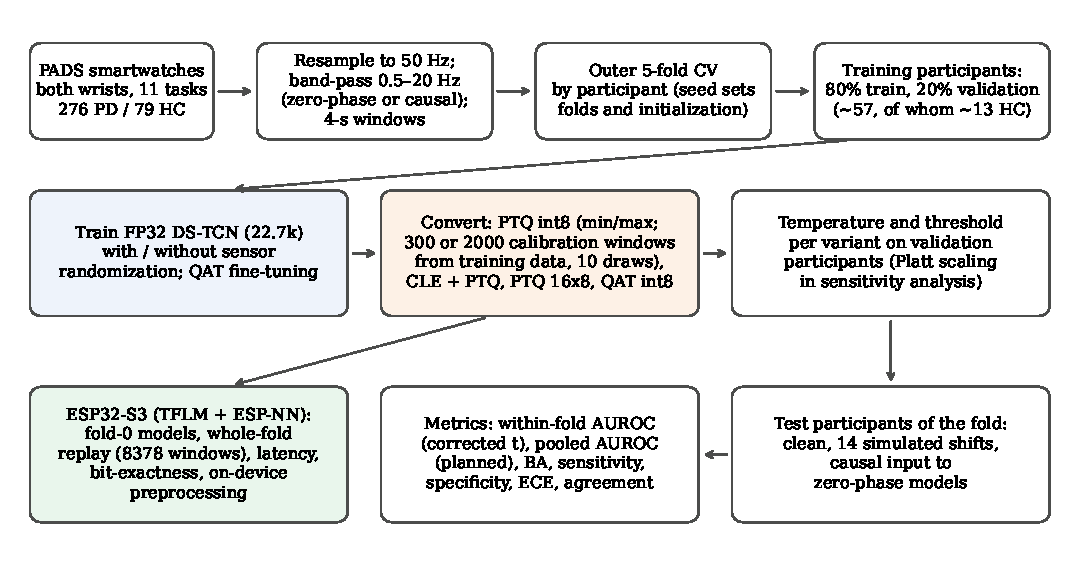
\includegraphics[width=\textwidth]{Figure_1.pdf}
\caption{Study pipeline. Calibration windows, temperatures and thresholds come from training participants only; test participants of each fold are used once for evaluation.}
\label{fig:pipeline}
\end{figure}

\subsection{Quantization variants}
Networks are trained with class-weighted binary cross-entropy, Adam (learning rate $10^{-3}$, batch 512) and up to 30 epochs, with early stopping (patience 6) on the window AUROC of validation participants. In each fold we build: FP32, the full-precision model; PTQ, a full-integer model (int8 input and output, per-channel weights, per-tensor activations) converted with TensorFlow Lite 2.21 using its default min/max range calibration on 300 training windows; and QAT, the FP32 weights fine-tuned for up to 5 epochs (learning rate $10^{-4}$, patience 3) with fake quantization (TensorFlow Model Optimization Toolkit 0.8.1, default 8-bit scheme, BN folded) before conversion. ``+SR'' variants repeat these steps for a model trained with sensor randomization: per batch, a uniformly random 3-D rotation of both sensors, a gain from 0.9 to 1.1, white noise with a standard deviation from 0 to 0.02~g or rad/s, and, with probability 0.25, the reflection mapping one wrist to the other. Every variant gets its own temperature and threshold on clean validation data, kept fixed under shift.

Exploratory variants were: PTQ calibrated on 2000 windows; PTQ of an FP32 model fine-tuned with the QAT schedule but without fake quantization; PTQ with int8 weights and int16 activations ($16\times8$); and PTQ after folding BN and applying CLE between each depthwise and pointwise convolution, which is exact here because no nonlinearity lies between them~\cite{NagelDFQ2019} (the folded models matched the original within $1.5\times10^{-5}$). To separate calibration-sample variance from training variance, each FP32 model of three seeds was converted ten more times with independently drawn 300- and 2000-window calibration sets, and fold 0 of seed 0 was retrained five times with different initializations. A layer-wise comparison of float and int8 activations used the TensorFlow Lite quantization debugger. To test the range mechanism, ten further retrainings of fold 0 (five each for seeds 0 and 1; runs q0 and q1) were each converted with ten pairs of calibration draws in two forms: as drawn (default min/max) and with every input channel clipped to its 0.1th and 99.9th percentiles over 5000 normalized training windows, so that the converter's own min/max calibration sees no extreme input values. For every int8 model we recorded the input and output quantization scales and the fraction of test input values that fall outside the int8 range (input saturation). Finally, five cross-validation runs (zero-phase runs t0--t2 for seeds 0--2 and causal runs u0--u1 for seeds 0--1; 25 fold models) converted each fold model with ten 300- and ten 2000-window draws, each as drawn and clipped at three percentile pairs (0.01/99.99, 0.1/99.9 and 1/99). Training on Kaggle CPUs was deterministic for a fixed script and seed: runs t0--t2 reproduced the weights and every result of r0--r2 exactly, so their min/max draws are the same conversions as in the draw analysis and the clipped conversions form exact pairs with them. Runs u0--u1 differ from k0--k1 after fold 0 because the earlier script consumed the random state differently, and are new models. To examine the mechanism and to measure fidelity without relying on about 16 test controls, fold 0 was retrained five more times for each of seeds 2 and 3 (runs v0 and v1; ten models), and each model was converted with ten min/max draws and the same draws clipped at 0.1/99.9 and 1/99. For every conversion we recorded the quantization scale of every activation tensor and, on the test windows, the root-mean-square difference between int8 and FP32 logits, the agreement of window decisions (sign of the logit) with FP32 and the window-level AUROC (about 8400 windows). Two selection rules used only the validation participants of each fold: choosing the clipping level with the highest mean validation AUROC over its draws, and choosing the single min/max draw with the highest validation AUROC. Analysis and firmware code were written with the assistance of a large language model (see the declaration at the end); all key statistics were recomputed with independently written scripts from the stored per-fold result files.

\subsection{Simulated sensor shifts and filter mismatch}
Shifts are applied to the raw 100-Hz test signals before preprocessing: resampling to 50 or 25~Hz (resampled back to 50~Hz, so the 25-Hz condition has no content above 12.5~Hz); timing jitter of 10\% or 30\% of the sampling period; a different accelerometer, simulated by adding gravity in a random direction, clipping to $\pm4$ or $\pm2$~g, quantizing to 12, 10 or 8 bits and removing gravity; white noise of 0.005 or 0.02~g and rad/s; rotations of both sensors by 15\textdegree, 45\textdegree\ or 180\textdegree; reflection to the other wrist; and removal of the gyroscope. The 50-Hz condition equals clean data and was kept in the planned 14-shift mean. The simulation does not model frequency response, anti-aliasing or clock drift~\cite{CoyleAsbil2026}, and the random gravity direction exaggerates clipping relative to seated tasks. Separately, zero-phase-trained models were evaluated on causally filtered test signals (filter mismatch).

\subsection{Statistical analysis}
We report participant-level AUROC, balanced accuracy (BA), sensitivity, specificity, expected calibration error (ECE, 10 bins) and agreement (fraction of decisions identical to the FP32 parent). Pooled AUROC is computed on predictions concatenated over five folds with 2000 participant-level bootstrap resamples stratified by class; within-fold AUROC is computed in each test fold (15 or 16 HC) and averaged.

\emph{Planned analysis.} The plan fixed three hypotheses on PD versus HC, tested on pooled predictions with paired bootstrap and Holm adjustment within each seed~\cite{Holm1979}: H1, PTQ is non-inferior to FP32 on clean data (margin $-0.02$ AUROC, one-sided); H2, quantization increases the mean AUROC loss over the 14 shifts; H3, QAT with SR gives a higher mean AUROC over the 14 shifts than PTQ. H2 and H3 were stated directionally but tested with two-sided bootstrap $p$ values, which is conservative; all CIs are two-sided percentile bootstrap intervals. Seed 0 was primary and seeds 1 and 2 were committed replications; no rule across seeds was defined. H3 compares two factors at once (training method and sensor randomization); the factorial within-fold contrasts in Table~\ref{tab:quant} separate them.

\emph{Exploratory analyses.} We repeated the planned contrasts after rank-normalizing scores within each fold and after Platt scaling (logistic regression of the validation logits, with intercept). Within-fold differences are summarized over fold--seed units with the corrected repeated $k$-fold $t$ statistic~\cite{Nadeau2003,Bouckaert2004} (variance factor $1/n + 0.25$, $n-1$ degrees of freedom), separately for each architecture and filter. Equivalence within $\pm0.02$ is examined with two one-sided tests at $\alpha=0.05$, which corresponds to the 90\% CI lying within the margin; equivalence results are given with 90\% CIs and all other CIs are 95\%. Exploratory $p$ values and confidence intervals (CIs) are unadjusted and descriptive.

\subsection{Runs}
\label{sec:runs}
Table~\ref{tab:fam} lists the run families and where each is reported. A run is one five-fold cross-validation (or, for q and v, five retrainings of fold 0) with a given seed; runs with the same seed use the same folds.

\begin{table}[!t]
\caption{Run families of the specified network.}
\label{tab:fam}
\centering\scriptsize
\setlength{\tabcolsep}{2.5pt}
\begin{tabular}{@{}llll@{}}
\toprule
Runs & Filter, seeds & Purpose & Reported in \\
\midrule
a & zero-phase, 0 & planned primary run & Tables~\ref{tab:hyp}, \ref{tab:runs}, \ref{tab:board} \\
z0--z2 & zero-phase, 0--2 & replication with the specified network & Table~\ref{tab:runs}; device replay (z0) \\
r0--r2 & zero-phase, 0--2 & as z, calibration stored; 10 draws per model & Tables~\ref{tab:runs}--\ref{tab:dec}, Figs.~\ref{fig:shift}, \ref{fig:draws} \\
k0--k2 & causal, 0--2 & device-matched filter & Tables~\ref{tab:runs}, \ref{tab:quant}, \ref{tab:board}; streaming (k0) \\
t0--t2 & zero-phase, 0--2 & identical to r0--r2, plus clipped draws & Table~\ref{tab:clip} \\
u0--u1 & causal, 0--1 & new causal models, clipped draws & Table~\ref{tab:clip} \\
q0--q1, v0--v1 & zero-phase, 0--3 & fold 0 retrained 5$\times$; ranges, fidelity & Section~\ref{sec:calib} \\
\bottomrule
\end{tabular}

\vspace{2pt}\parbox{\linewidth}{\footnotesize Benchmark networks and feature models (Table~\ref{tab:main}) come from a separate seed-0 run. Five runs with a script error (no BN after the depthwise convolutions) are reported in Supplementary Table~S1.}
\end{table}

\subsection{On-device deployment}
\label{sec:device}
Models run on an ESP32-S3 module (dual-core Xtensa LX7 at 240~MHz, 16~MB flash, 8~MB octal PSRAM) with ESP-IDF v5.3.2, TensorFlow Lite for Microcontrollers (esp-tflite-micro) and ESP-NN kernels; the tensor arena is in internal SRAM, and its use is read with \texttt{arena\_used\_bytes}. A benchmark firmware replays 50 test windows and checks every output byte against the reference interpreter. A second firmware receives windows over USB and returns the output and inference time, which we used to replay every window of the fold-0 test participants (zero-phase seed-0 models) and compute participant-level AUROC from on-device outputs. Two further firmwares run the whole preprocessing chain on the device, per window and as a stream, and a random forest (100 trees, depth 8) runs with emlearn~\cite{emlearn}.

% =====================================================================
\section{Results}
\label{sec:results}
\subsection{Benchmark (RQ1)}
Feature models were at least as accurate as every network (Table~\ref{tab:main}). For PD versus HC, the paired within-fold difference was $+0.024$ AUROC for the random forest over the DS-TCN (95\% CI $-0.029$ to $+0.076$) and $+0.036$ for XGBoost ($-0.001$ to $+0.074$). For PD versus DD, all networks stayed below the feature models. With a random window-level split, the window AUROC rose from 0.748 to 0.862 for PD versus HC and from 0.639 to 0.827 for PD versus DD, which shows the size of leakage. Varghese et al.~\cite{Varghese2024} reported mean balanced accuracies of 91.2\% (PD versus HC) and 72.4\% (PD versus DD) for their models under a different protocol that included age matching; because we report participant-level AUROC on all participants, the figures are not directly comparable, but both studies find PD versus DD much harder. For PD versus HC, pooled AUROC was 0.001 to 0.045 lower than within-fold AUROC for the networks and 0.003 to 0.005 lower for the feature models, whose probabilities were not temperature-scaled per fold (Section~\ref{sec:pool}).

\begin{table}[!t]
\caption{Participant-level benchmark (seed 0; separate benchmark run, so the DS-TCN values differ from those of the quantization runs in Table~\ref{tab:runs}): pooled AUROC (95\% bootstrap CI) and within-fold AUROC, mean (SD over folds).}
\label{tab:main}
\centering\scriptsize
\setlength{\tabcolsep}{2.5pt}
\begin{tabular}{@{}lccccc@{}}
\toprule
 & & \multicolumn{2}{c}{PD vs HC} & \multicolumn{2}{c}{PD vs DD} \\
\cmidrule(lr){3-4}\cmidrule(lr){5-6}
Model & Params & Pooled & Within fold & Pooled & Within fold \\
\midrule
Random forest & -- & 0.900 (0.860--0.937) & 0.905 (0.025) & 0.757 & 0.758 (0.036) \\
XGBoost & -- & 0.915 (0.882--0.945) & 0.918 (0.014) & 0.723 & 0.725 (0.027) \\
DS-CNN & 11.1k & 0.825 (0.772--0.873) & 0.861 (0.041) & 0.685 & 0.689 (0.037) \\
1-D CNN & 32.2k & 0.833 (0.783--0.876) & 0.878 (0.026) & 0.661 & 0.693 (0.043) \\
CNN-LSTM & 44.6k & 0.839 (0.790--0.883) & 0.864 (0.044) & 0.652 & 0.676 (0.035) \\
DS-TCN & 22.7k & 0.856 (0.807--0.901) & 0.882 (0.023) & 0.635 & 0.681 (0.119)$^{a}$ \\
DS-TCN, invariant input & 22.7k & 0.807 (0.756--0.856) & 0.846 (0.062) & 0.633 & 0.624 (0.124)$^{a}$ \\
DS-TCN, attention pooling & -- & 0.846 (0.796--0.889) & 0.847 (0.048) & 0.551 & 0.566 (0.019) \\
\bottomrule
\end{tabular}

\vspace{2pt}\parbox{\linewidth}{\footnotesize Networks: one seed. Feature models, seeds 1 and 2 (PD vs HC, pooled): random forest 0.908 and 0.912, XGBoost 0.888 and 0.918. $^{a}$One fold near chance.}
\end{table}

\subsection{Planned hypotheses (RQ2, RQ3)}
\label{sec:planned}
Seeds 1 and 2 of the planned replication were first executed by a script in which the BN after each depthwise convolution had been disabled (21,841 parameters; Section~\ref{sec:dev}); they were re-run with the specified architecture, and these runs are used here. On pooled predictions (Table~\ref{tab:hyp}), H1 was supported in seed 1 only, H2 in no seed and H3 in seeds 0 and 1. After per-fold rank normalization, H1 was not shown in any seed, H2 remained null and H3 was not supported in any seed after Holm adjustment. The planned confirmatory evidence is therefore inconclusive.

\begin{table}[!t]
\caption{Planned hypotheses (PD versus HC, zero-phase filter): pooled predictions as planned, and after per-fold rank normalization (exploratory). CIs are unadjusted.}
\label{tab:hyp}
\centering\scriptsize
\setlength{\tabcolsep}{2.5pt}
\begin{tabular}{@{}llcccc@{}}
\toprule
 & & \multicolumn{2}{c}{Pooled (planned)} & \multicolumn{2}{c}{Fold-normalized} \\
\cmidrule(lr){3-4}\cmidrule(lr){5-6}
H & Seed & Estimate (95\% CI) & $p_\text{Holm}$ & Estimate (95\% CI) & $p_\text{Holm}$ \\
\midrule
H1 & 0 & $-0.063$ ($-0.112$, $-0.012$) & 0.96 & $-0.088$ ($-0.140$, $-0.038$) & 1.00 \\
 & 1 & $+0.036$ ($+0.001$, $+0.074$) & \textbf{0.005} & $-0.014$ ($-0.035$, $+0.008$) & 0.81 \\
 & 2 & $-0.041$ ($-0.073$, $-0.010$) & 1.00 & $-0.015$ ($-0.037$, $+0.006$) & 0.95 \\
H2 & 0 & $+0.008$ ($-0.006$, $+0.023$) & 0.62 & $+0.000$ ($-0.012$, $+0.013$) & 1.00 \\
 & 1 & $+0.003$ ($-0.009$, $+0.014$) & 0.58 & $+0.004$ ($-0.004$, $+0.012$) & 0.81 \\
 & 2 & $+0.003$ ($-0.006$, $+0.012$) & 1.00 & $+0.004$ ($-0.006$, $+0.014$) & 0.95 \\
H3 & 0 & $+0.133$ ($+0.058$, $+0.210$) & \textbf{$<$0.001} & $+0.058$ ($+0.003$, $+0.117$) & 0.14 \\
 & 1 & $+0.055$ ($+0.011$, $+0.099$) & \textbf{0.030} & $-0.008$ ($-0.040$, $+0.024$) & 0.81 \\
 & 2 & $+0.000$ ($-0.079$, $+0.073$) & 1.00 & $+0.003$ ($-0.028$, $+0.037$) & 0.95 \\
\bottomrule
\end{tabular}

\vspace{2pt}\parbox{\linewidth}{\footnotesize H1: PTQ$-$FP32, clean; $p$ one-sided against the $-0.02$ margin. H2, H3: two-sided bootstrap $p$. H2: loss of PTQ minus loss of FP32 (clean minus 14-shift mean). H3: QAT+SR minus PTQ, 14-shift mean. Bold: supported.}
\end{table}

\subsection{Why the pooled estimand failed}
\label{sec:pool}
The planned estimand was poorly chosen for this protocol. In the three additional zero-phase runs, where calibration parameters were stored, the fitted FP32 temperatures ranged from 0.12 to the upper search bound of 20 (reached in 4 of 15 folds), and the median raw participant logit varied between folds from $-0.86$ to $+1.99$. Temperature scaling has no intercept, so it cannot remove such offsets, and with about 13 validation controls per fold the temperature itself is poorly determined. The pooled FP32 AUROC was 0.716 to 0.813, whereas the within-fold AUROC was 0.856 to 0.885. Platt scaling with an intercept, fitted on the same validation participants, raised the pooled AUROC to 0.832 to 0.880, close to the within-fold values (for QAT, 0.845 to 0.889). The pooling problem is known~\cite{Forman2010,Airola2011,Fawcett2006}; here it reversed the sign of the planned PTQ contrast in one seed. All further results are within-fold.

\subsection{Quantization within folds (exploratory)}
Quantization did not interact with sensor shift: the within-fold difference in shift-induced loss between PTQ and FP32 (the H2 contrast, clean minus the 14-shift mean) was $+0.002$ (90\% CI $-0.012$ to $+0.017$; equivalent within $\pm0.02$, $p=0.023$) with zero-phase filtering (runs r0--r2) and $+0.003$ ($-0.006$ to $+0.012$; $p=0.002$) with causal filtering (runs k0--k2). Excluding the 50-Hz condition, which equals clean data, gave the same estimates (equivalence $p=0.032$ and $0.004$). The margin of 0.02 AUROC was chosen as a difference too small to change a screening decision at the precision these cohorts allow; it is not a clinically validated threshold. Table~\ref{tab:runs} lists every run and Table~\ref{tab:quant} summarizes the specified network.

PTQ with 300 calibration windows lost on average 0.028 (zero-phase) and 0.017 (causal) AUROC, with CIs that include zero, but single folds lost up to 0.089, and the planned seed-0 run lost 0.087 on average (0.219 in one fold), whereas its repeat lost 0.010. A 2000-window calibration set gave a larger average loss (0.054 and 0.055) and worse single folds (up to 0.254). CLE did not help ($-0.033$; worst fold $-0.248$), and PTQ of a sensor-randomized model failed badly in one fold ($-0.368$). In contrast, $16\times8$ quantization was equivalent to FP32 in every unit (largest loss 0.009; $p<0.001$ in both settings), and QAT showed no average loss ($+0.005$ and $0.000$; worst fold $-0.039$). Across the 50 fold-run units of the specified network, PTQ lost more than 0.05 in 12 and QAT in 2; the SDs were 0.040 and 0.024. Because runs with the same seed share folds (z and r runs are repeats), these units are not independent and we did not test the difference in spread; per run, PTQ had more folds losing more than 0.05 than QAT in four of the seven zero-phase runs (QAT had more in one) and in two of the three causal runs, and equally many in the rest.

\begin{table}[!t]
\caption{Within-fold clean AUROC of FP32 and mean difference from FP32 (worst fold) for every run of the specified network, PD versus HC.}
\label{tab:runs}
\centering\scriptsize
\setlength{\tabcolsep}{2pt}
\begin{tabular}{@{}lllccccc@{}}
\toprule
Run & Filter & Seed & FP32 & PTQ int8 & PTQ, 2000 & PTQ $16\times8$ & QAT int8 \\
\midrule
\multicolumn{8}{@{}l}{\emph{Specified network (BN after depthwise convolutions)}} \\
a & Zero-phase & 0 (planned) & 0.879 & $-0.087$ ($-0.219$) & -- & -- & $+0.004$ ($-0.035$) \\
z0 & Zero-phase & 0 & 0.868 & $-0.010$ ($-0.020$) & $-0.045$ & $+0.002$ & $0.000$ ($-0.058$) \\
z1 & Zero-phase & 1 & 0.881 & $-0.013$ ($-0.051$) & $-0.041$ & $+0.001$ & $-0.004$ ($-0.033$) \\
z2 & Zero-phase & 2 & 0.867 & $-0.015$ ($-0.052$) & $-0.031$ & $-0.001$ & $-0.025$ ($-0.052$) \\
r0 & Zero-phase & 0 & 0.861 & $-0.022$ ($-0.039$) & $-0.100$ & $+0.001$ & $-0.004$ ($-0.039$) \\
r1 & Zero-phase & 1 & 0.885 & $-0.038$ ($-0.078$) & $-0.051$ & $-0.001$ & $+0.011$ ($-0.033$) \\
r2 & Zero-phase & 2 & 0.856 & $-0.023$ ($-0.083$) & $-0.012$ & $-0.001$ & $+0.008$ ($-0.039$) \\
k0 & Causal & 0 & 0.875 & $0.000$ ($-0.018$) & $-0.024$ & $0.000$ & $-0.003$ ($-0.018$) \\
k1 & Causal & 1 & 0.856 & $-0.028$ ($-0.060$) & $-0.041$ & $-0.002$ & $+0.005$ ($-0.012$) \\
k2 & Causal & 2 & 0.849 & $-0.024$ ($-0.089$) & $-0.100$ & $0.000$ & $-0.001$ ($-0.027$) \\
\bottomrule
\end{tabular}

\vspace{2pt}\parbox{\linewidth}{\footnotesize Each row is one cross-validation run (five folds), identified by the run label used in all other tables and figures; runs with the same seed share folds. Runs r0--r2 repeat z0--z2 with calibration parameters stored. Five runs affected by a script error (no BN after the depthwise convolutions) are listed in Supplementary Table~S1. Worst fold: most negative of the five fold differences.}
\end{table}

\begin{table}[!t]
\caption{Within-fold AUROC difference from the reference for the specified network (runs r0--r2 for the zero-phase filter and k0--k2 for the causal filter, 15 fold--seed units each; 95\% CI from the corrected $t$).}
\label{tab:quant}
\centering\scriptsize
\setlength{\tabcolsep}{2.5pt}
\begin{tabular}{@{}lcccc@{}}
\toprule
 & \multicolumn{2}{c}{Zero-phase filter} & \multicolumn{2}{c}{Causal (device) filter} \\
\cmidrule(lr){2-3}\cmidrule(lr){4-5}
Variant & Mean (95\% CI) & Worst & Mean (95\% CI) & Worst \\
\midrule
FP32 (AUROC) & 0.867 & -- & 0.860 & -- \\
PTQ int8, 300 windows & $-0.028$ ($-0.066$, $+0.010$) & $-0.083$ & $-0.017$ ($-0.055$, $+0.020$) & $-0.089$ \\
PTQ int8, 2000 windows & $-0.054$ ($-0.135$, $+0.027$) & $-0.254$ & $-0.055$ ($-0.121$, $+0.011$) & $-0.174$ \\
PTQ int8 after CLE & $-0.033$ ($-0.110$, $+0.045$) & $-0.248$ & -- & -- \\
PTQ of fine-tuned FP32$^{a}$ & $-0.035$ ($-0.092$, $+0.023$) & $-0.161$ & $-0.023$ ($-0.069$, $+0.024$) & $-0.103$ \\
PTQ $16\times8$ & $0.000$ ($-0.004$, $+0.004$) & $-0.009$ & $-0.001$ ($-0.004$, $+0.003$) & $-0.005$ \\
QAT int8 & $+0.005$ ($-0.026$, $+0.037$) & $-0.039$ & $0.000$ ($-0.019$, $+0.020$) & $-0.027$ \\
FP32 + SR & $-0.022$ ($-0.061$, $+0.017$) & $-0.074$ & $-0.028$ ($-0.070$, $+0.013$) & $-0.078$ \\
PTQ + SR$^{b}$ & $-0.031$ ($-0.146$, $+0.084$) & $-0.368$ & $+0.001$ ($-0.029$, $+0.031$) & $-0.036$ \\
QAT + SR & $-0.019$ ($-0.064$, $+0.026$) & $-0.085$ & $-0.025$ ($-0.065$, $+0.016$) & $-0.090$ \\
\bottomrule
\end{tabular}

\vspace{2pt}\parbox{\linewidth}{\footnotesize $^{a}$Relative to the fine-tuned FP32 model. $^{b}$Relative to FP32 + SR. Worst: most negative unit.}
\end{table}

At the decision level (Table~\ref{tab:dec}), PTQ lowered BA and sensitivity, while QAT and $16\times8$ kept BA within 0.01 of FP32. Agreement with FP32 decisions was 80\% for PTQ, 85\% for QAT and 99\% for $16\times8$; a merely fine-tuned FP32 model agreed in 91\%, so part of the disagreement comes from refitting thresholds on few controls. Expected calibration errors of 0.12 to 0.15 after temperature scaling are high, consistent with the poorly determined temperatures discussed in Section~\ref{sec:pool}. SR lowered clean AUROC and did not improve the shift mean; it helped only for a 180\textdegree\ rotation (FP32 + SR 0.849 versus FP32 0.777) and hurt most without the gyroscope (0.780 versus 0.840; Fig.~\ref{fig:shift}).

\begin{table}[!t]
\caption{Clean decision metrics (runs r0--r2, mean over 15 fold--seed units). Decisions use the threshold refitted for each variant on validation participants.}
\label{tab:dec}
\centering\footnotesize
\begin{tabular}{@{}lcccccc@{}}
\toprule
Variant & AUROC & BA & Sensitivity & Specificity & ECE & Agreement \\
\midrule
FP32 & 0.867 & 0.775 & 0.780 & 0.770 & 0.146 & 1.000 \\
PTQ int8 & 0.839 & 0.724 & 0.711 & 0.737 & 0.145 & 0.802 \\
PTQ int8 after CLE & 0.835 & 0.749 & 0.742 & 0.755 & 0.136 & 0.832 \\
PTQ $16\times8$ & 0.867 & 0.768 & 0.782 & 0.754 & 0.146 & 0.989 \\
QAT int8 & 0.873 & 0.778 & 0.759 & 0.797 & 0.124 & 0.854 \\
QAT + SR & 0.848 & 0.758 & 0.783 & 0.734 & 0.144 & 0.867 \\
FP32 fine-tuned & 0.877 & 0.761 & 0.807 & 0.715 & 0.122 & 0.910 \\
\bottomrule
\end{tabular}
\end{table}

\begin{figure}[!t]
\centering
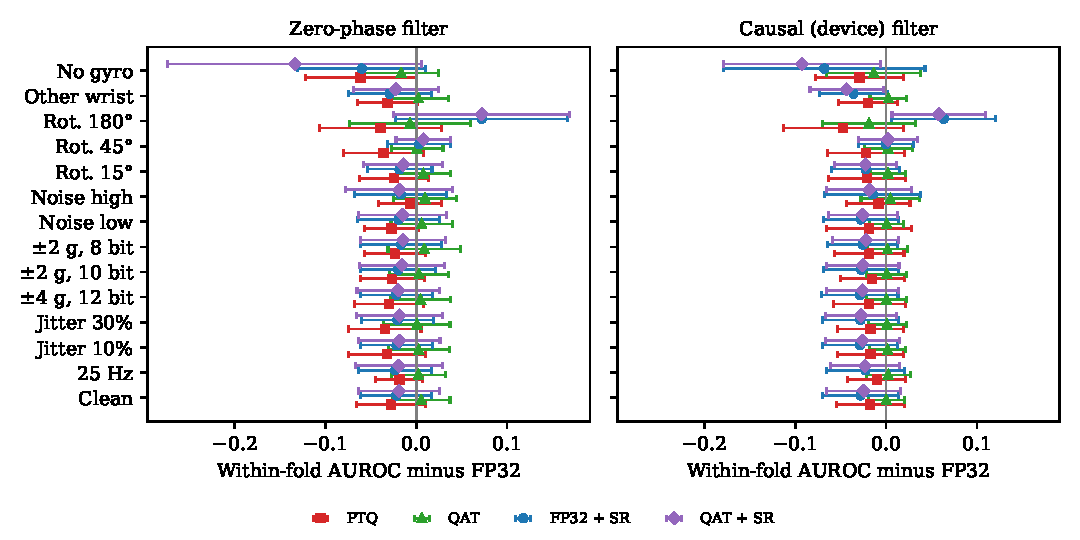
\includegraphics[width=\textwidth]{Figure_2.pdf}
\caption{Within-fold AUROC difference from FP32 under each simulated shift (runs r0--r2; mean and 95\% corrected-$t$ CI over 15 fold--seed units). The 50-Hz condition equals clean data and is not shown.}
\label{fig:shift}
\end{figure}

\subsection{Calibration-sample sensitivity}
\label{sec:calib}
Fig.~\ref{fig:draws} shows the 150 additional conversions of the 15 zero-phase FP32 models. With 300 windows, the loss averaged 0.032, exceeded 0.05 in 23\% of draws and reached 0.220. The SD across draws of the same model (0.033) was larger than the SD of the per-model means (0.020), so most of the variation came from the calibration sample rather than from the trained weights. With 2000 windows, the loss was not smaller (mean 0.038; 27\% of draws above 0.05; worst 0.299), as expected for min/max ranges, which can only widen as more windows are seen~\cite{Wu2020}. In the five retrainings of fold 0, the FP32 AUROC ranged from 0.874 to 0.914; default PTQ changed it by $-0.040$ to $+0.042$, single calibration draws by $-0.106$ to $+0.028$ and CLE by $-0.082$ to $+0.018$, whereas $16\times8$ stayed within 0.002 and QAT within $-0.006$ to $+0.021$.

Across all folds, clipping removed almost all large losses (Table~\ref{tab:clip}). In the 25 fold models of runs t0--t2 and u0--u1, default min/max calibration lost 0.029 (300 windows) and 0.042 (2000 windows) on average, and 22\% and 30\% of draws lost more than 0.05, up to 0.220 and 0.327. With the 1/99 percentiles these shares fell to 1.2\% and 0.4\%, the mean losses to 0.002 and 0.004 and the worst draws to 0.065 and 0.089; 0.1/99.9 was almost as good, and 0.01/99.99 helped only partly. Clipping at 0.1/99.9 reduced the per-model mean loss in 22 of 25 models for each calibration size (Wilcoxon $p<0.001$), and the improvement was positive in each of the five runs; because t0--t2 share seeds and folds with r0--r2, the zero-phase and causal runs are the two groups that are independent of each other, and both showed the effect (zero-phase 13 of 15 models, $p\le0.003$; causal 9 of 10, $p\le0.02$). Choosing the clipping level on validation data (1/99 in 33 of 50 choices) gave a mean loss of 0.004 and a worst model of 0.065. Choosing the best min/max draw on validation helped with 300 windows (mean 0.007, 4\% of models losing more than 0.05) but not with 2000 windows (0.022, 12\%). Balanced accuracy was 0.765 for FP32, 0.730 and 0.725 with min/max calibration and 0.751 and 0.742 with clipping at 0.1/99.9; agreement of decisions with FP32 rose from 0.82 and 0.79 to 0.87 and 0.86. In the same runs, $16\times8$ changed AUROC by at most 0.009, QAT averaged $+0.004$ (worst $-0.039$) and CLE did not help (mean $-0.029$ over these 25 models, worst $-0.248$).

\begin{table}[t]
\caption{Calibration strategies for default int8 PTQ: AUROC change from FP32 over 25 fold models (runs t0--t2, u0--u1), ten calibration draws per model and setting.}
\label{tab:clip}
\centering\scriptsize
\setlength{\tabcolsep}{3pt}
\begin{tabular}{@{}lcccccc@{}}
\toprule
 & \multicolumn{3}{c}{300 windows} & \multicolumn{3}{c}{2000 windows} \\
\cmidrule(lr){2-4}\cmidrule(lr){5-7}
Calibration & Mean & $>0.05$ loss & Worst & Mean & $>0.05$ loss & Worst \\
\midrule
Min/max (default) & $-0.029$ & 22.4\% & $-0.220$ & $-0.042$ & 29.6\% & $-0.327$ \\
Clipped 0.01/99.99 & $-0.020$ & 12.4\% & $-0.158$ & $-0.027$ & 22.4\% & $-0.172$ \\
Clipped 0.1/99.9 & $-0.005$ & 0.8\% & $-0.105$ & $-0.009$ & 2.4\% & $-0.132$ \\
Clipped 1/99 & $-0.002$ & 1.2\% & $-0.065$ & $-0.004$ & 0.4\% & $-0.089$ \\
\midrule
Clip level chosen on validation$^a$ & $-0.004$ & -- & $-0.065$ & $-0.004$ & -- & $-0.058$ \\
Best min/max draw on validation$^a$ & $-0.007$ & 4\% & $-0.067$ & $-0.022$ & 12\% & $-0.077$ \\
\bottomrule
\end{tabular}

\smallskip
\parbox{\linewidth}{\scriptsize $^a$One choice per fold model; percentages are shares of models. Draw-level noise: some draws gained up to 0.066 AUROC over FP32.}
\end{table}

The range measurements on the ten retrained fold-0 models of runs q0 and q1 (FP32 AUROC 0.830 to 0.919) showed that the loss is not caused by input saturation. With default min/max calibration, at most 0.005\% of test input values saturated, and across draws the loss was not correlated with the input scale (Spearman $\rho=-0.03$ for 300 windows and $+0.14$ for 2000 windows) or with the output scale. Over 100 draws per setting, the loss averaged 0.023 (300 windows) and 0.051 (2000 windows), exceeded 0.05 in 15\% and 41\% of draws and reached 0.207 and 0.317. Clipping the same draws at the 0.1/99.9 input percentiles made the input scale three to five times finer (0.074 versus 0.224 and 0.338), saturated 0.07\% of test input values, and reduced the mean loss to 0.010 and 0.009, the share of draws losing more than 0.05 to 2\% and the worst draw to 0.059 and 0.057. The worst draw of every model was within 0.06 with clipping, against up to 0.207 (300 windows) and 0.317 (2000 windows) without it, and the improvement in the per-model mean loss was clearest for 2000 windows (better in 9 of 10 models, Wilcoxon $p=0.006$; 300 windows, 7 of 10, $p=0.19$). In the same models, $16\times8$ changed AUROC by at most 0.003 and QAT by $-0.022$ to $+0.030$. Some draws gained up to 0.065 AUROC over FP32, and FP32 AUROC itself varied by about 0.04 between retrainings with the same folds; with about 16 controls per test fold, a single-draw difference below about 0.05 is within evaluation noise, which is why we report the share of draws exceeding 0.05. The ten models of runs v0 and v1 (FP32 AUROC 0.783 to 0.892) reproduced the pattern and showed where it acts. With min/max calibration, 17\% (300 windows) and 31\% (2000 windows) of draws lost more than 0.05 participant AUROC, against 0 to 2\% with clipping; window-level AUROC, which rests on about 8400 windows, fell by 0.049 and 0.068 on average with min/max calibration and by 0.012 and 0.013 with clipping at 1/99, and window decisions agreed with FP32 in 79\% and 71\% of windows against 91\% and 90\%. Within a model, draws with a larger logit error lost more participant AUROC (Spearman $\rho=-0.40$) and the window- and participant-level losses were correlated ($\rho=+0.51$), so the participant-level losses are not artefacts of the small number of test controls. Min/max calibration produced activation scales 1.6 to 2.2 times larger than clipped calibration in the convolutional and residual layers, 1.4 times larger after pooling and 1.2 times at the output, and the input scale 5.5 times larger. Within a model, larger scales went with larger losses in every layer ($\rho=-0.16$ to $-0.36$ for min/max draws), most strongly in the first pointwise convolutions and the first residual additions and least in the output layer. 16$\times$8 changed participant AUROC by at most 0.005, and QAT by $-0.030$ to $+0.039$. The layer-wise comparison in fold 0 showed rounding errors near the uniform value of 0.29 quantization steps in most layers after the stem and 0.44 to 0.66 steps in the stem, which also quantizes the input; within a layer, the largest channel range was at most 8.4 times the median. No single layer explained the loss.

\begin{figure}[!t]
\centering
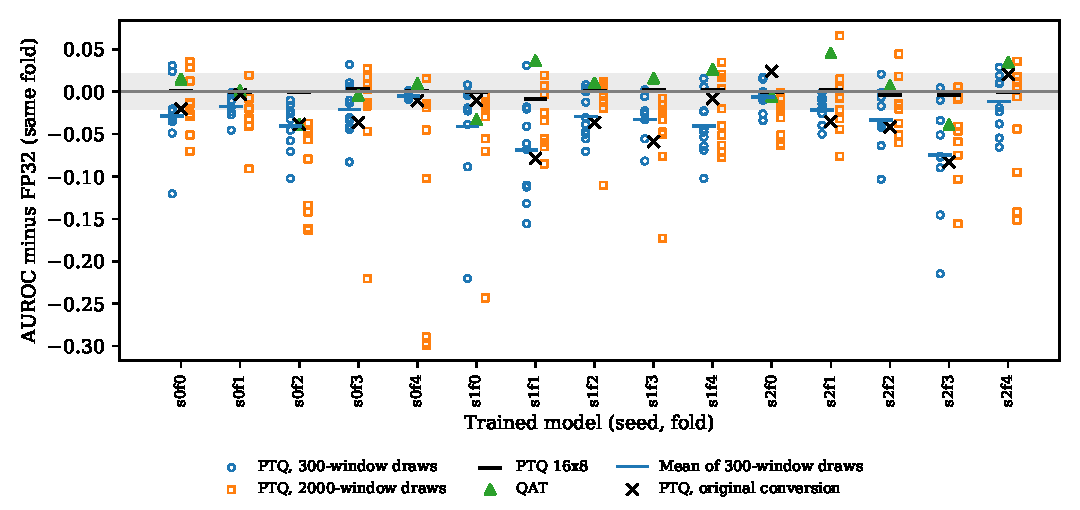
\includegraphics[width=\textwidth]{Figure_3.pdf}
\caption{PTQ loss for ten independent calibration draws of 300 and 2000 training windows per trained model (15 models of runs r0--r2: seed s, fold f; cross: the original conversion reported in Table~\ref{tab:runs}; blue line: mean of the 300-window draws), with $16\times8$ quantization and QAT of the same model for comparison. Grey band: $\pm0.02$.}
\label{fig:draws}
\end{figure}

\subsection{Filter mismatch}
When zero-phase-trained models were fed causally filtered test signals, the within-fold AUROC fell by 0.020 for FP32 (95\% CI $-0.048$ to $+0.007$), 0.044 for QAT ($-0.093$ to $+0.006$) and 0.043 for PTQ, with single folds losing up to 0.159. Models trained with the causal filter reached 0.860 (FP32 and QAT) on causal input. For the deployed random forest, zero-phase training with causal features lost 0.017 ($-0.041$ to $+0.007$), and causal training recovered it ($+0.002$). All CIs include zero, so the mismatch effect is suggestive rather than established; it was smaller for the feature model.

\subsection{Confounding by age and sex}
Within each sex, the FP32 network kept most of its discrimination (rank-normalized AUROC 0.79 to 0.84 in women and 0.85 to 0.89 in men across six runs). Age and sex alone gave a within-fold AUROC of 0.68 to 0.69, and adding the network score raised it to 0.85 to 0.88.

\subsection{On-device measurements}
Replaying the complete fold-0 test set (71 participants, 8378 windows) through the ESP32-S3 gave outputs identical to the desktop reference interpreter for 8373 windows (QAT) and 8374 windows (PTQ), the rest being one least significant step apart, and participant-level AUROCs of 0.889 (QAT) and 0.856 (PTQ), identical to the desktop values (Table~\ref{tab:board}). The same replay with the fold-0 models of the specified causal run k0, fed causally filtered windows as on the device, gave 8371 (QAT) and 8372 (PTQ) identical outputs and device AUROCs of 0.884 and 0.908, again identical to the desktop. Inference took 10.7~ms per window (0.5\% of the 2-s step between overlapping windows). The $16\times8$ model took 562.5~ms per window, about 49 times longer than the int8 model in the same 50-window benchmark (11.6~ms), because ESP-NN has no int16 kernels for these operators. A streaming firmware with persistent filter states, run with the fold-0 QAT model of the specified causal run k0, classified a 4-s window every 2~s in 12.6~ms per step (1.0~ms preprocessing per 2-s block, 0.7~ms normalization and quantization, 10.9~ms inference) with 40.3~kB of RAM (22.6~kB arena), and its outputs were bit-exact with a causal Python pipeline on all 27 windows of three recordings. Together with the whole-fold replays, this validates the on-device preprocessing chain and the integer inference of the deployable causal model; the whole-fold replays used host-side causal filtering, whose equivalence to the firmware filter rests on the 27-window streaming test. The deployed random forest (100 trees, depth 8, causal features) reached an AUROC of 0.923 in fold 0 and 0.898 across the five folds; it took 2.5~ms per participant, and the 96 features of one 10-s recording took 10.5~ms.

\begin{table}[!t]
\caption{Network inference on the ESP32-S3 (240 MHz, fold-0 models, ESP-NN kernels unless noted).}
\label{tab:board}
\centering\scriptsize
\setlength{\tabcolsep}{2.5pt}
\begin{tabular}{@{}lccccc@{}}
\toprule
Model (test set) & ms & Arena kB & Model kB & Identical & AUROC dev./desk. \\
\midrule
PTQ int8 (50 win.) & 11.56 & 21.2 & 49.5 & 50/50 & -- \\
PTQ int8, portable (50 win.) & 70.29 & 20.2 & 49.5 & 50/50 & -- \\
QAT int8 (50 win.) & 11.54 & 21.2 & 50.9 & 50/50 & -- \\
QAT int8 (whole fold) & 10.68 & 22.6 & 50.9 & 8373/8378 & 0.889/0.889 \\
PTQ int8 (whole fold) & 10.68 & 22.6 & 49.5 & 8374/8378 & 0.856/0.856 \\
QAT int8, causal (whole fold) & 10.68 & 22.6 & 50.9 & 8371/8378 & 0.884/0.884 \\
PTQ int8, causal (whole fold) & 10.69 & 22.6 & 49.5 & 8372/8378 & 0.908/0.908 \\
PTQ $16\times8$ (50 win.) & 562.5 & 27.8 & 58.1 & 46/50 & -- \\
\bottomrule
\end{tabular}

\vspace{2pt}\parbox{\linewidth}{\footnotesize Whole fold: 71 participants, 8378 windows (run z0; causal rows: run k0 with causally filtered input); 50-window tests: run a and, for $16\times8$, run z0. The four non-identical $16\times8$ outputs differ by one step of the int16 output scale, as expected from fixed-point rounding in the reference (non-ESP-NN) kernels. Non-identical outputs differ by one least significant step. Model: flatbuffer size; 1~kB = 1000 bytes. Latency: mean of 1000, 8378 or 100 ($16\times8$) invocations.}
\end{table}

% =====================================================================
\section{Discussion}
\label{sec:discussion}
The planned analysis did not answer its questions, and the reason is methodological. We chose pooled AUROC with per-fold temperature scaling as the primary estimand; with about 13 validation controls per fold, temperatures were ill-determined and fold offsets remained, so pooled values of the same model ranged widely and reversed the sign of one planned contrast. The plan was therefore mis-specified. Platt scaling or per-fold evaluation removed the problem. Studies that pool cross-validated predictions after per-fold calibration on small validation sets should check within-fold metrics as well~\cite{Forman2010,Airola2011,Varoquaux2018}.

The quantization results apply to TensorFlow Lite's default min/max calibration. For this network, its outcome depended mainly on which training windows were drawn for calibration: the same trained model lost nothing with one draw and more than 0.1 AUROC with another, and larger calibration sets did not help. Min/max ranges are set by the most extreme activations seen, so a calibration set that includes a few atypical windows coarsens the eight-bit grid for all others; 16-bit activations, which are far less sensitive to range, removed the loss. CLE, which balances weight ranges, did not address this. That outliers dominate min/max ranges and that clipping helps is known from general quantization work~\cite{Wu2020,Banner2019ACIQ,Zhao2019OCS}; our contribution is to quantify how much it matters, and how variable it is, for a small clinical wearable network evaluated per participant. Clipping the calibration windows at the 1/99 or 0.1/99.9 input percentiles, a pre-processing step that needs no change to the converter, removed almost all large losses in every fold, and the level can be chosen on validation data. Input saturation was negligible and the input scale itself did not predict the loss, whereas the activation scales of the internal layers did: extreme calibration windows widen the ranges of all layers by a factor of about two, which coarsens the eight-bit grid throughout the network, and the draws that widen them most lose most. The effect is distributed over the network rather than located in one layer, which is consistent with the absence of a single culprit in the layer-wise comparison. Window-level AUROC and logit agreement, which do not depend on the few test controls, showed the same pattern, so a label-free check of logit agreement with FP32 on a few thousand windows is a practical way to screen a conversion. Selecting the best of several min/max draws on validation is a weaker remedy, because with about 13 validation controls per fold the selection itself is noisy. Per-layer percentile, entropy or mean-squared-error ranges and adaptive rounding~\cite{Wu2020,Nagel2020AdaRound} were not compared and may do better. A single conversion with default min/max calibration is weak evidence that a quantized wearable model is safe: in our runs, almost a quarter of calibration draws lost more than 0.05 AUROC. QAT showed no average loss and usually fewer large losses than PTQ, though not in every run (in run z0 its worst fold was worse) and the difference in spread was not significant for the specified network; it cost nothing on the device and kept decisions closer to FP32; a 16-bit model is not a practical alternative on this microcontroller, because it ran about 49 times slower.

Two device-level points matter as much as quantization. First, preprocessing must match: zero-phase filtering cannot run in real time, and models trained with it tended to lose AUROC on causally filtered signals (CIs including zero, single folds up to 0.159), whereas causally trained models did not. Second, bit-exact kernels allow desktop results to stand for device results: a complete fold replayed on the board reproduced the desktop AUROC exactly. Filtering also determines how equivalent the raw signals of different accelerometers are~\cite{CoyleAsbil2026}, which our simulated shifts did not capture.

The benchmark puts the network in context. Feature models were at least as accurate, needed no quantization and also ran on the microcontroller. The random forest, however, scores a participant only after all 22 task--wrist recordings are available, whereas the network gives a score for every 4-s window of one wrist, which is what continuous or single-task monitoring needs; whether that advantage holds in practice was not tested here. Our quantization findings concern one small network and one converter and should not be generalized to other architectures without checking. Both the network and the feature models used both wrists and all eleven tasks, which requires two watches and a supervised protocol; whether a single-wrist, reduced-task configuration remains accurate was not tested and is needed before either is used on one wearable.

\subsection{Deviations from the analysis plan}
\label{sec:dev}
(i) The executed network placed the downsampling stride in the depthwise rather than the pointwise convolution of blocks two and four; the parameter count and the receptive field (127 input samples, 2.5~s at 50~Hz) are unchanged, but the depthwise convolutions of these blocks see every second position and activation statistics may differ from the planned design. (ii) The first runs of seeds 1 and 2, the initial device-matched runs, an earlier per-window firmware (Supplementary Section~S3) and an external-cohort analysis used a script in which the BN after each depthwise convolution had been disabled; the quantization runs and the streaming firmware test were repeated with the specified network (Table~\ref{tab:runs}), and the external-cohort analysis was not repeated. Its results (seven external controls, CIs too wide to inform any comparison) are given in Supplementary Section~S2. (iii) Fold-normalized, Platt-scaled, within-fold, calibration-draw and device-matched analyses were added after the first results.

\subsection{Limitations}
Calibration was varied only through the input windows; per-layer range estimators and adaptive rounding were not compared. Shifts were simulated, and no external cohort with a different device was analysed. One architecture family and one microcontroller were studied, the benchmark networks used one seed, and runs with the same seed differ when the script changed the random state, so replicate runs differ by seed rather than by repetition. Within-fold AUROC rests on about 16 controls per fold. The cohort comes from a referral clinic, with more women among controls; network scores retained discrimination within each sex, but we did not match on age or sex. Energy was not measured with a suitable instrument, so we make no energy claims.

% =====================================================================
\section{Conclusions}
\label{sec:conclusion}
For a 22.7k-parameter network detecting Parkinson's disease from wrist inertial signals, planned tests of eight-bit quantization on pooled cross-validated predictions were inconclusive because temperature-only calibration on small validation sets made pooling unstable. Within folds, the shift-induced loss of quantized and full-precision models was equivalent within $\pm0.02$ AUROC. Default post-training quantization was unreliable: its loss depended mainly on the calibration sample and was not reduced by larger calibration sets or cross-layer equalization, whereas clipping the calibration inputs at their 1/99 or 0.1/99.9 percentiles removed almost all large losses in 25 fold models. Sixteen-bit activations removed the loss but were about 49 times slower on an ESP32-S3, whereas quantization-aware training showed no average loss at no on-device cost. A complete test fold replayed on the device reproduced the desktop AUROC, and training with the device's causal filter may avoid a filter-mismatch loss that was suggested but not established. For small wearable networks like this one, calibration inputs should be clipped or quantization-aware training used, conversions should be checked across calibration draws, and evaluations should use per-fold metrics and the device's own preprocessing.

% =====================================================================
\section*{CRediT authorship contribution statement}
\textbf{Quang-Tuyen Lai:} Conceptualization, Methodology, Software, Investigation, Formal analysis, Data curation, Visualization, Writing -- original draft. \textbf{Ba-Viet Ngo:} Conceptualization, Methodology, Supervision, Validation, Writing -- review \& editing.

\section*{Declaration of competing interest}
The authors declare that they have no known competing financial interests or personal relationships that could have appeared to influence the work reported in this paper.

\section*{Funding}
This research did not receive any specific grant from funding agencies in the public, commercial, or not-for-profit sectors.

\section*{Ethics statement}
This study used only the publicly available, de-identified PADS dataset~\cite{PADSdata}, accessed from PhysioNet under its published licence and terms of use. No new data were collected from human participants, so no additional ethical approval was required.

\section*{Data and code availability}
PADS is available from PhysioNet~\cite{PADSdata}. The training, evaluation and conversion code, fold assignments, per-fold result files, firmware and the dated analysis plan with its amendment log will be released in a public repository when the article is published.

\section*{Declaration of generative AI and AI-assisted technologies in the manuscript preparation process}
During the preparation of this work the authors used Claude (Opus 5.5, Anthropic) in order to assist with writing analysis and firmware code, running the statistical analyses, and drafting and editing the manuscript. Key statistics were recomputed with separately written scripts from the stored per-fold result files, and firmware outputs were checked against reference implementations (bit-exactness tests and a whole-fold replay). After using this tool, the authors reviewed and edited the content as needed and take full responsibility for the content of the published article.

\bibliographystyle{elsarticle-num}
\bibliography{refs}

\end{document}
